\documentclass{article}
\usepackage{graphicx}
\usepackage{textcomp}
\usepackage{amssymb}
\usepackage[utf8]{inputenc}
\usepackage[T1]{fontenc}
\usepackage{amsmath}
\usepackage{pgfplots}
\usepackage{tikz}
\usepackage{hyperref}
\usepackage{apacite}
\pgfplotsset{compat=1.18}

\usepackage{setspace}
\doublespacing


\title{Predictive Analytics: Soccer Performance Data
and All-SEC Honors}
\author{Caleb Reid}
\date{May 12, 2025}

\begin{document}
\maketitle

\section{Abstract}
All-SEC awards are highly valuable to D1 women's soccer players but are difficult to earn. Using a binary variable to denote players in the top 10 of performance metrics, provided by Wyscout, a predictive model can be created to analyze what metrics contribute the most to earning a spot on an All-SEC team. An elastic net classification model was created to calculate odds ratios and predict out-of-sample performance. The most influential metric was goalsPer90 (OR = 83.6\%) followed by shotsPer90 (OR = 41.4\%). The model correctly predicted 6/9 All-SEC athletes in the test set (sensitivity = 0.44) and had a moderate agreement with the outcome varaible, allSEC, (kappa = 0.48). Future research should incorporate performance data for all athletes in the SEC, not just those in the top 10 of each respective performance metric.

\section{Introduction}
Each year the Southeastern Conference (SEC) recognizes the top performing student-athletes in NCAA Division I (D1) women’s soccer with its All-SEC teams. The top performing athletes from the regular season are placed in three teams: first-team, second-team, or third-team, with first-team All-SEC being the most prestigious honor. The awards are voted on by the league’s 16 coaches following the conclusion of the regular season \cite{sec2025}.

To better understand how student-athletes can earn these awards, an analytical approach is needed. Wyscout, the largest soccer data and video database in the world \cite{wyscout}, provides performance data to every university in the SEC. Using Wyscout performance data, a predictive model can be created to analyze what metrics lead to earning a spot on an All-SEC team. 

\section{Literature Review}
The SEC is a NCAA D1 athletic conference that consists of 16 teams since the addition of Oklahoma and Texas in 2024. All-SEC awards are a highly prestigious honor that can propel an athlete’s career. Earning an All-SEC selection can increase the odds of playing professional soccer, which are very slim odds. Only 1\% of NCAA women’s soccer players will play professional soccer once they graduate \cite{howManyPlayers2025}which is lower than the chance of making it to the NFL! (1.6\%) \cite{cesconetto2021}. While there has not been research into how many All-SEC women’s soccer players play professionally, any chance to improve your 1\% odds should be pursued.

Research into how All-SEC teams are selected and how to predict awards is essentially nonexistent. The research question was prompted by a SEC women’s soccer coach who wanted to know what his players’ Wyscout stats need to be in order to earn an All-SEC selection. The coach’s question demonstrates the lack of research in the topic, and highlights the ambiguity surrounding how athletes are selected for All-SEC.

Despite the lack of research in All-SEC teams, there has been studies conducted on the performance data provided by Wyscout, albeit limited. Previous research has explored the relationship between match performance indicators (MPI), collected by Wyscout, and Global Positioning System (GPS) data in D1 women’s soccer \cite{sam2023}. A statistically significant relationship was found between hard running distance (HRD) and MPIs (0.639 $\leq$ r $\leq$ 0.992). This study is encouraging because it shows that Wyscout data may be informative beyond relative game performance across an SEC regular season. GPS data is one of the most commonly used tools for athlete tracking and monitoring in D1 women’s soccer, highlighting the significance of this study. However, despite the encouragement of this study, it is only one study. More research is needed to validate the use of GPS data to predict performance metrics in Wyscout. 

Furthermore, the relationship between visual tracking speed (VTS) and performance data, collected by Wyscout, in SEC women’s soccer \cite{phillips2022,phillips2023}. \citeA{phillips2022} discovered that the relationship between VTS and passing accuracy was nonsignificant ($r$  = -0.380). Furthermore, \citeA{phillips2023} did not find any significant differences in performance metrics after a three-dimensional motion object tracking (3D-MOT) training intervention ($p$ > 0.05). While not related to All-SEC honors, these studies provide a framework for analyzing Wyscout performance metrics. However, the lack of significant findings suggest that the performance metrics may not be predictive of VST or future performance. 
In conclusion, All-SEC awards are a valuable marker of success and could potentially increase a D1 women’s soccer player’s odds of making it to a professional league. However, no literature exists exploring the relationship between all-SEC awards, or any NCAA awards for that matter, and performance data provided by Wyscout. Previous research has found a relationship between performance metrics and GPS data, which is encouraging but not widely validated. Furthermore, Wyscout performance data has not been found to be a good predictor of VST or future performance. Therefore, the purpose of this study is to build a predictive model using Wyscout performance metrics to predict All-SEC selection.

\section{Data}
\subsection{Team Rosters}
A sample of 1,283 SEC women’s soccer players was compiled over three SEC regular seasons, 2023-2025. The sample included every SEC women’s soccer player from past three season, minus goalkeepers and unidentifiable players. For each athlete, name, year, team, and position (pos) were identified. The rosters were scraped from each SEC teams’ website using the rvest package in RStudio (version 2026.01.2+418A). Athletes from the 2023 Oklahoma and Texas rosters were excluded due to the fact they were ineligible to receive an All-SEC selection; OU and Texas did not join the SEC until the summer of 2024. 

\subsection{All-SEC}
SEC award information was collected from secsports.com from 2023-2025 \cite{sec2023,sec2024,sec2025}. The categories of interest were first, second, or third-team All-SEC. Initially, All-Freshman Team was included as an All-SEC award, but it was excluded from the model due to the fact that only freshman are eligible to receive a selection on the All-Freshman team. Athletes were denoted by 1 if they earned an All-SEC recognition for that season and a 0 if not.

\subsection{Wyscout}
Wyscout player data is only provided for athletes who finished among the top 10 of a given performance metric in the SEC regular season. This poses a significant missing data problem, as most athletes in the SEC player database will not have any data, even if they played significant minutes. Therefore, for each individual season, a nominal binary variable [0,1] was assigned to each athlete based on their inclusion in the top 10 of each Wyscout performance metric, where 1 means they were among the top 10 in the category and 0 means they were not. Table 1 shows the three data sources used to compile the final dataset.

Wyscout provides attacking and defensive metrics, but no performance metrics were provided for goalkeepers, which is why they were excluded from this study. Attacking metrics include goalsPer90, assistsPer90, shotsPer90, keyPassesPer90, and touchesBoxPer90. Defensive metrics included defDuelsPer90, aerialDuelsPer90, interceptionsPer90, recoveriesPer90, slidingTacklesPer90, and shotsBlockedPer90. There are 90 minutes in an D1 women’s soccer game, so metrics are shown on a per 90 minutes played basis.

\subsection{Final Dataset}
The final dataset included one dependent variable: allSEC, one unique identifier: id, and 14 predictor variables: year, team, pos, and the 11 performance metrics mentioned above. Table 2 shows an overview of the data.

\section{Methods}
Before creating a predictive model, the final dataset was cleaned to ensure validity of the dataset. All athletes were placed into four positions: forward (F), midfield (M), defense (D), or multiple. Many athletes were listed as playing multiple positions, and instead of forcing athletes into one category, a new position was created: multiple. A summary table (table 3) was created to showcase the number of All-SEC selections earned by each position. Despite having a fewer number of observations, the athletes who played multiple positions made up 7.4\% of the All-SEC selections while the average rate across all positions was 5.8\%, demonstrating the exclusivity of All-SEC teams. 

To explore the relationship between Wyscout performance metrics and All-SEC selection, an elastic net classification model was created using the glm package in RStudio. 

\[
\log\left(
\frac{P(\text{allSEC}=1)}
{1-P(\text{allSEC}=1)}
\right)
=
\beta_0
+
\sum_{j=1}^{13}\beta_j X_j
\]

{\footnotesize
\[
X_j \in \{\text{year, pos, goalsPer90, assistsPer90, shotsPer90,}
\]
\[
\text{keyPassesPer90, touchesBoxPer90, defDuelsPer90,}
\]
\[
\text{aerialDuelsPer90, recoveriesPer90, interceptionsPer90,}
\]
\[
\text{slidingTacklesPer90, shotsBlockedPer90}\}
\]
}

All variables were binary, except year and pos, which were transformed into factors. The dataset was split into training (80\%) and test (20\%) sets. Additionally, the training set was split using five-fold cross validation. Due to the low number of positive observations, the model was stratified on allSEC to ensure even distribution of the folds. The model was tuned to determine the appropriate mixture of ridge and LASSO, with the final mixture equal to 0.75. Cohen’s Kappa was used to determine the appropriate tuning parameter $\lambda$, with the final value of $\lambda$ equal to 0.037. Accuracy alone is not an appropriate metric for determining model performance, due to class imbalance in the outcome variable; most observations will result in allSEC = 0. As mentioned above, only 5.8\% of athletes are chosen for All-SEC teams, so a model that predicts all athletes as not making an All-SEC team would have an accuracy of 94.2\%.
To test the model’s out-of-sample performance, a confusion matrix was created (table 4). The optimal cutoff was determined using Cohen’s Kappa, with the final value of the predicted class being 0.42.

\section{Findings}
The results of the elastic net classification model returned beta coefficients for each of the predictor variables. Using the exponential form of these coefficients, the odds ratio for each variable can be calculated to determine the predictive power each variable has on allSEC. The top 9 most influential variables are included in fig. 1.

From this plot, it is clear that goalsPer90 is by far the most influential factor in determining All-SEC selection. Placing in the top 10 of goalsPer90, over the course of a SEC regular season, results in a 83.6\% better chance of earning a place on an All-SEC team compared to another athlete who was not included in the top 10. The next most important factor is shotsPer90, with a 41.4\% increase in likelihood of earning an All-SEC honor if included in the top 10. In fact, the top 3 most influential factors are all attacking stats (goalsPer90, assistsPer90, keyPassesPer90). This is reflective of the positional breakdown from above, which showed that defenders had the worst average placement in All-SEC teams (4.2\%) of all positions. However, defense was not entirely overlooked as the next three most influential factors were all defending stats, with slidingTacklesPer90 (14.2\%) and aerialDuelsPer90 (12.1\%) being the top two predictors of allSEC. 

To test the model’s performance on out-of-sample data, i.e. test data, a confusion matrix was created (table 4). The model had a kappa of 0.48, which is a moderate strength of agreement \cite{landis1977}, and a sensitivity metric of 0.44, which means it correctly predicted 44\% of positive cases. The model correctly identified 244/248 non-All-SEC athletes and 6/9 All-SEC athletes. 

\section{Conclusion}
The odds ratio plot (fig. 1) showed that attacking stats are the most important in determining All-SEC selection. This coincides with the positional breakdown table that showed that forwards and midfielders, positions that get the most attacking stats, are more likely to earn All-SEC honors. Furthermore, goalsPer90 being the most influential variable is to no surprise. Goals help you win games and scoring a lot of goals in a given year will certainly gain the attention of coaches across the SEC. Being amongst the top 10 of goals (per 90 mins) increases your chance of being selected to an All-SEC team by a whopping 84\%. Therefore, to maximize the likelihood of earning a spot on an All-SEC teams, attacking players should look to score as many goals as possible. It is important to note that defensive performance metrics were also valued highly, but no metric came close to goalsPer90.
In terms of model performance, the elastic net classification model is not a great predictor of All-SEC awards. Due to the amount of missing data, it is difficult to create a model that will accurately predict the All-SEC teams for a given year. The model had a moderate association with allSEC, but it cannot be used as a reliable measure for predicting All-SEC teams. It misidentified four non-All-SEC players and missed three All-SEC players. 

\subsection{Limitations}
The obvious limitation of this study is that Wyscout performance data is only provided for athletes who finished in the top 10 of the respective category. The amount of missing data required the variables to be transformed into binary variables, when continuous variables are more reflective of the actual data. Furthermore, the Wyscout data was in a .pdf form, which could negatively impact the validity of the data. The data was copied and pasted into a spreadsheet, but sometimes the data that is pasted does not match the data in the .pdf. Furthermore, the Wyscout data only provided first initial and last name, meaning that athletes with the same first initial, last name, team, and year are inseparable. These athletes had to be removed to increase the validity of the data. Another limitation of this study is that variables were chosen based off prior knowledge, not with any analytical technique. Lastly, this study is only generalizable to women’s soccer All-SEC teams, and cannot be used to assess any other NCAA all-conference awards.

\subsection{Future Research}
Future research in predicting All-SEC teams should include performance data for all athletes with the SEC, not just those in the top 10. This would solve the missing data issue, and give a better, more informative model. Another goal of future researchers should be to cross-validate variables to include in the model. Using a proven data science technique to choose variables would increase validity and predictive power of the model. Lastly, increasing the number of years of the study would give more examples for the model to train and test on, possibly increasing the Kappa and sensitivity of  the model on out-of-sample data.

\subsection{Final Thoughts}
While inclusion in the top 10 of a given performance record should theoretically give you a good chance of earning a place on one of the all-SEC teams, the reality is that there are many more factors that account for why an athlete is selected. The conference’s 16 coaches are responsible for voting on the awards, and past experiences with these athletes can cause bias in their decisions. For example, most of the coaches know the athletes in the conference as recruiting is very competitive in the SEC. Therefore, coaches have probably had interactions with these athletes and that could affect their decision come voting time. Their opinion of the athlete may be a larger factor in their decision making than the athlete’s performance. Furthermore, the Transfer Portal opens up opportunities for athletes to move schools at the end of the year, meaning that some athletes will have played for multiple SEC schools in their collegiate career. It is possible that some athletes may not receive a vote because the coach who recruited that athlete does not like that they left their school and joined another program within the conference.

\newpage

\bibliographystyle{apacite}
\bibliography{Reid_finalPaper}

\appendix

\section{Appendix}

\begin{table}[htbp]
  \centering
  \caption{Wyscout Example}
  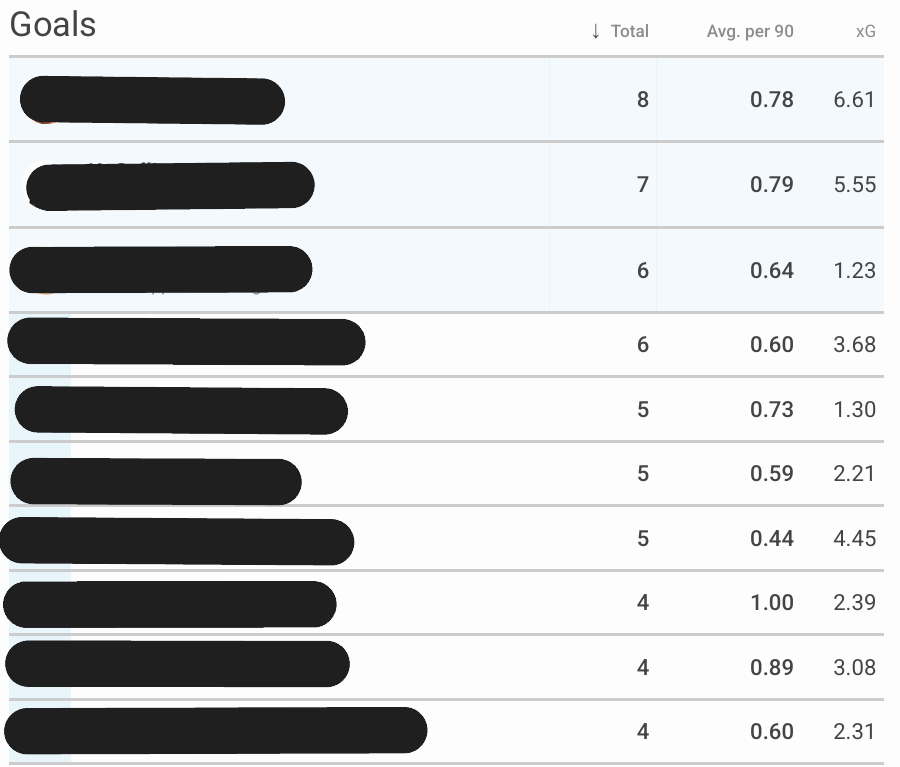
\includegraphics[width=\textwidth]{wyscoutExample.png}
  \label{tab:wyscout}
\end{table}

\begin{table}[htbp]
  \centering
  \caption{Data Overview}
  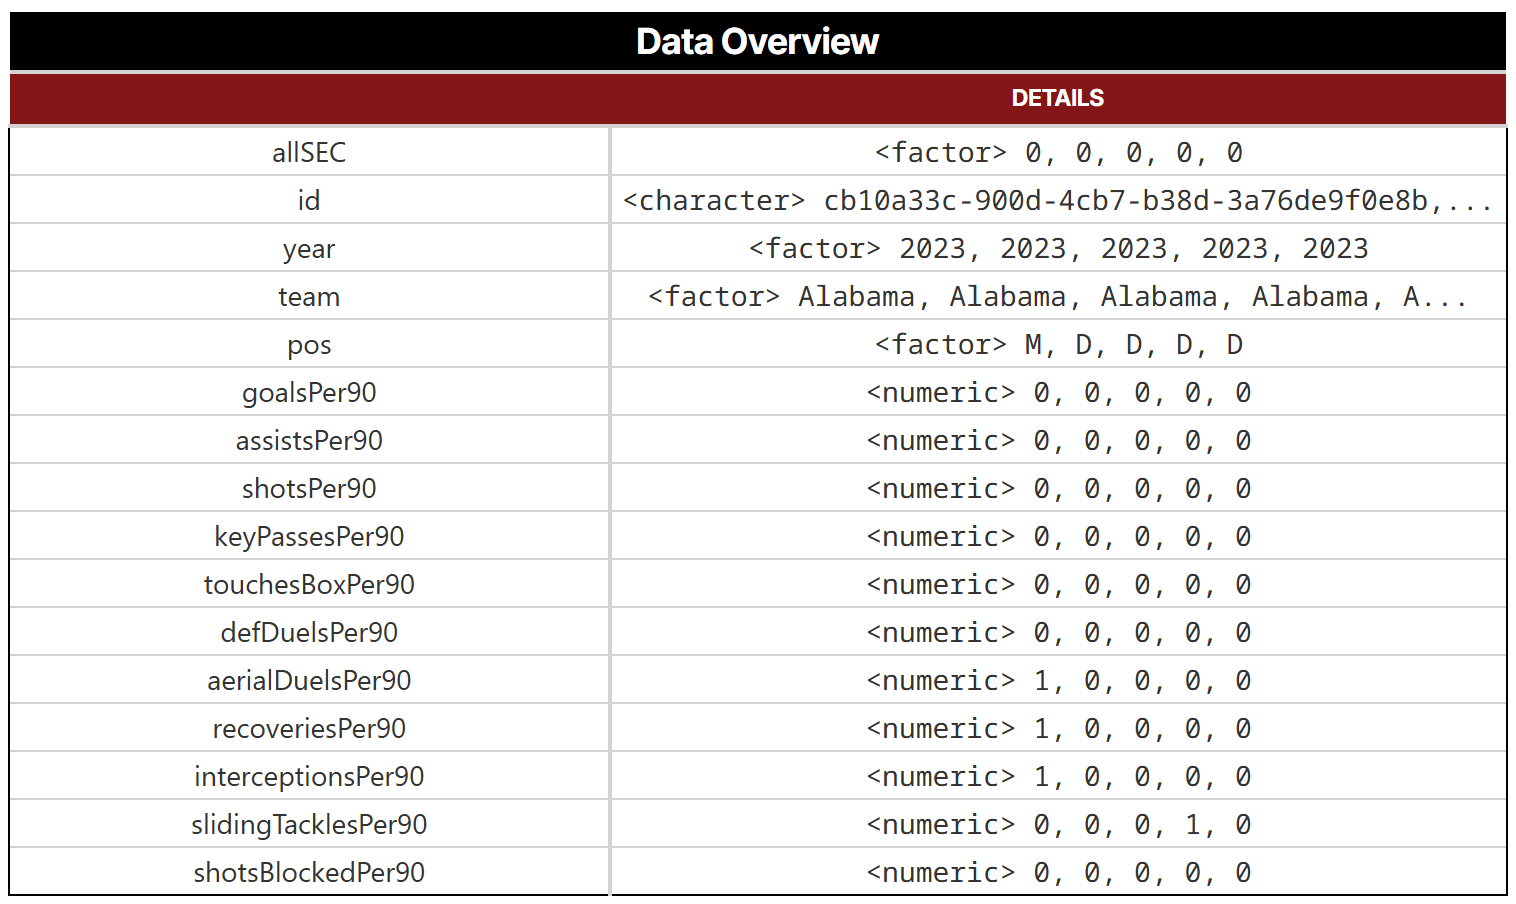
\includegraphics[width=\textwidth]{dataOverviewTable.png}
  \label{tab:dataoverview}
\end{table}

\begin{table}[htbp]
  \centering
  \caption{Position Breakdown}
  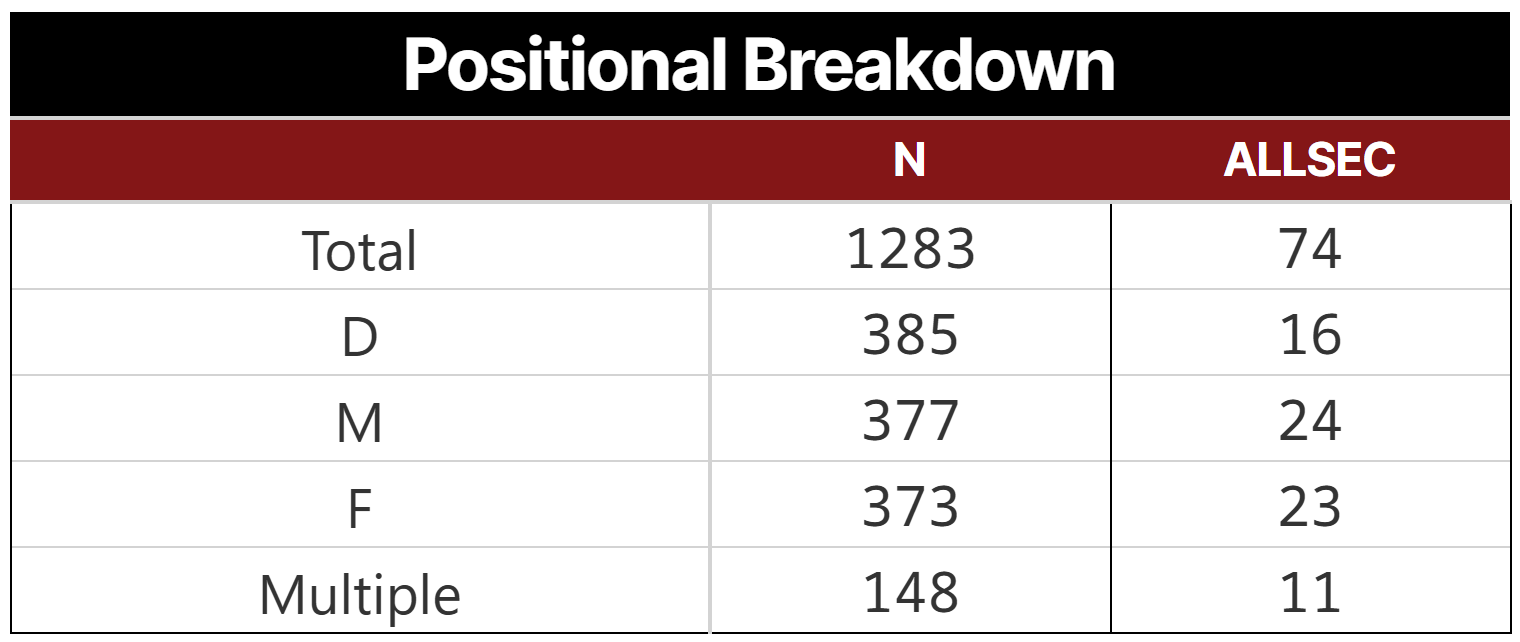
\includegraphics[width=\textwidth]{posBreakdown.png}
  \label{tab:posbreakdown}
\end{table}

\begin{table}[htbp]
  \centering
  \caption{Confusion Matrix}
  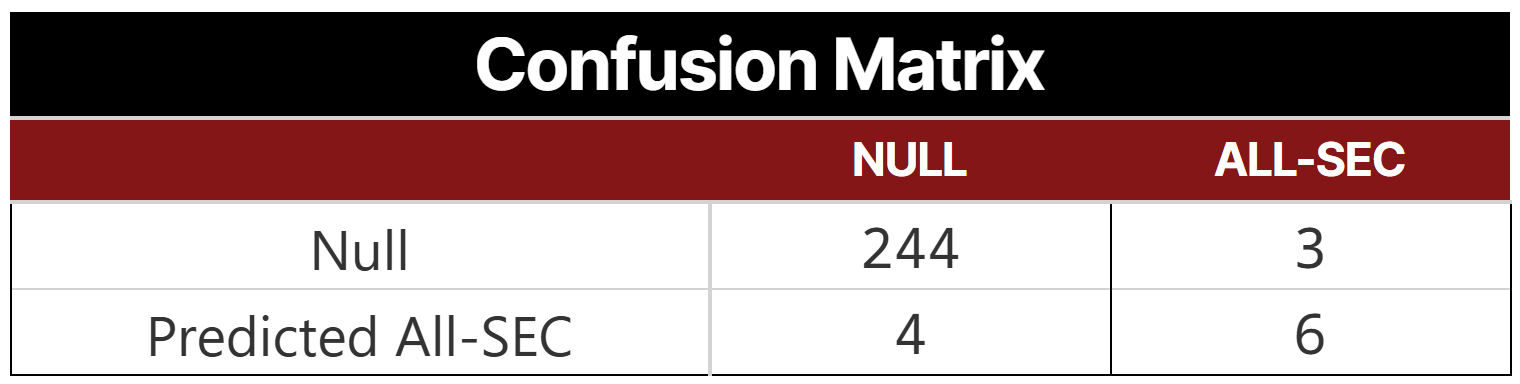
\includegraphics[width=\textwidth]{confusionMatrixGT2.png}
  \label{tab:confusion}
\end{table}

\begin{figure}[htbp]
  \centering
  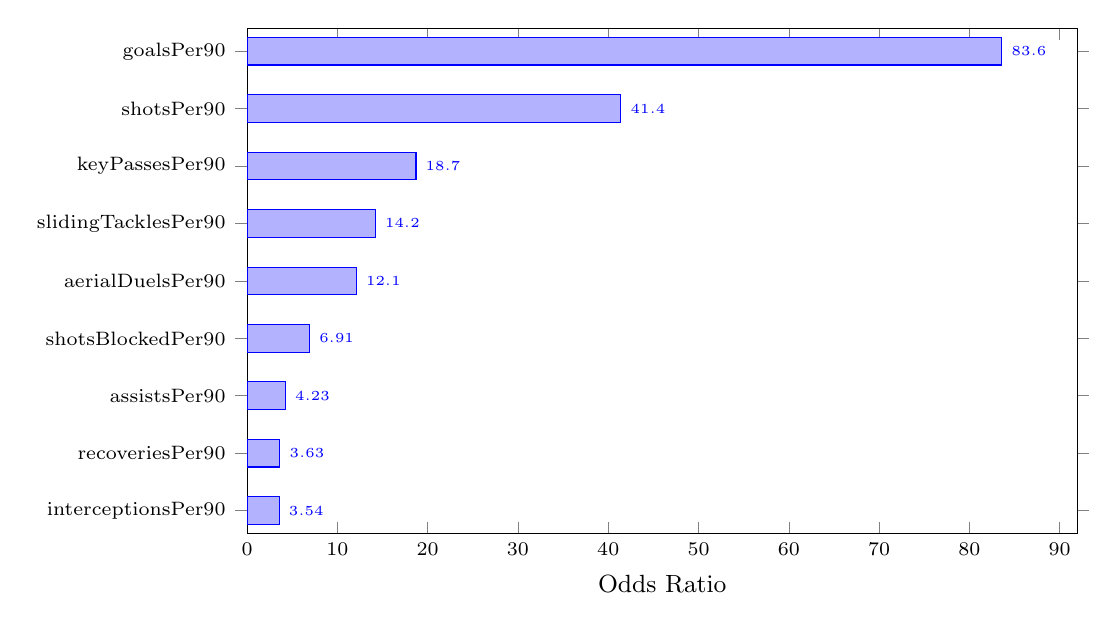
\begin{tikzpicture}
  \begin{axis}[
      xbar,
      width=\textwidth,
      height=8cm,
      xmin=0,
      xlabel={Odds Ratio},
      symbolic y coords={
          interceptionsPer90,
          recoveriesPer90,
          assistsPer90,
          shotsBlockedPer90,
          aerialDuelsPer90,
          slidingTacklesPer90,
          keyPassesPer90,
          shotsPer90,
          goalsPer90
      },
      ytick=data,
      nodes near coords,
      nodes near coords align={horizontal},
      enlarge y limits=0.05,
      tick label style={font=\scriptsize},
      label style={font=\small},
      every node near coord/.append style={font=\tiny}
  ]
  \addplot coordinates {
      (83.6,goalsPer90)
      (41.4,shotsPer90)
      (18.7,keyPassesPer90)
      (14.2,slidingTacklesPer90)
      (12.1,aerialDuelsPer90)
      (6.91,shotsBlockedPer90)
      (4.23,assistsPer90)
      (3.63,recoveriesPer90)
      (3.54,interceptionsPer90)
  };
  \end{axis}
  \end{tikzpicture}
  \caption{Odds Ratios of Significant Predictors}
  \label{fig:oddsratio}
\end{figure}

\end{document}